%!TEX root = TFG.tex

\chapter{Resultados} \label{chap:result}

Una vez entrenados todos los algoritmos con sus mejores hiperparámetros y con un valor de generalización obtenido de la predicción, se obtienen los resultados que se ven en la Fig. \ref{fig:comp_accur}.

\begin{figure}
    \centering
    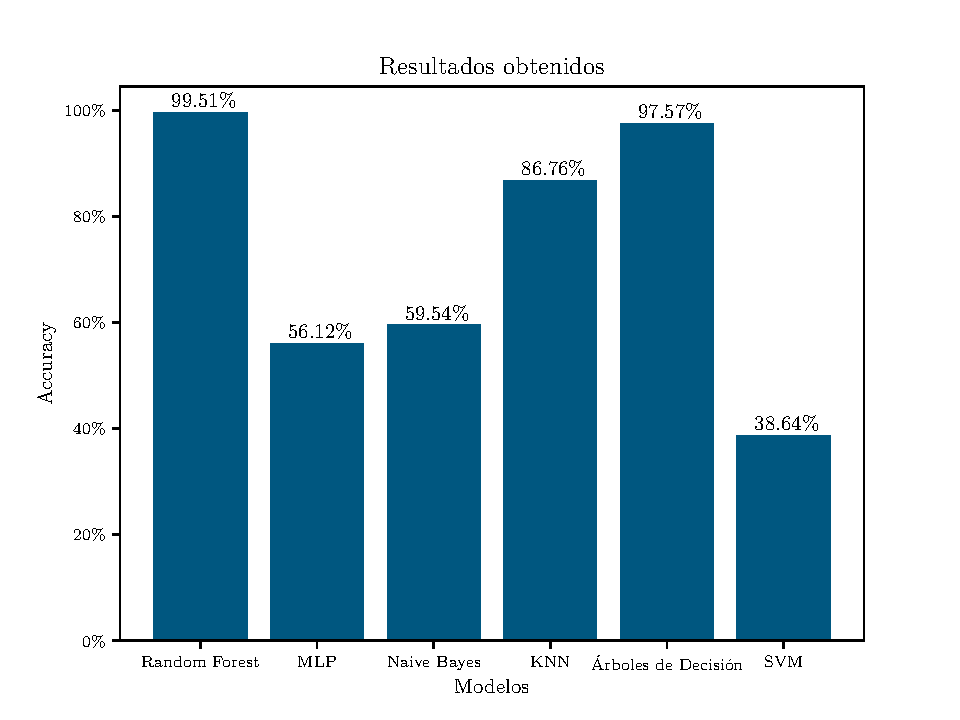
\includegraphics[width=0.6\textwidth]{../Python/plots/parallel/accur_results}
    \caption{Comparativa de resultados entre modelos}
    \label{fig:comp_accur}
\end{figure}

Como se puede ver en la figura anteriormente mencionada, los modelos que presentan mejores resultados son los que se basan en árboles de decisión, que son el propio algoritmo de árboles de decisión y random forest. Otra forma de ver estos resultados es mediante las matrices de confusión que genera cada algoritmo.

Una matriz de confusión es una tabla que evalúa los resultados de un modelo Machine Learning orientado a la clasificación. En este tipo de tablas se enfrentan valores bien predichos y mal predichos observando las etiquetas reales y las predichas por los datos. Un ejemplo de matriz de confusión se puede ver a continuación en la Tabla \ref{tab:ex_confusion_matrix}. Con este tipo de herramientas en sencillo ver los aciertos y fallos de un modelo. Esta herramienta también se puede generalizar a clasificación multiclase, que ha sido el uso en este trabajo.

Con una matriz de confusión es posible obtener las distintas métricas que sirven para comparar los modelos de Machine Learning como accuracy, recall o F-score.

\begin{multicols}{2}
\begin{equation}
    Accuracy = \frac{TP + TN}{TP + FP + FN + TN}
\end{equation}
\begin{equation}
    Recall = \frac{TP}{TP + FN}
\end{equation}
\begin{equation}
    F-score = \frac{2 \cdot TP}{2 \cdot TP + FP + FN}
\end{equation}
\end{multicols}

\begin{table}
    \centering
    \begin{tabular}{@{}cc cc@{}}
        \multicolumn{1}{c}{} &\multicolumn{1}{c}{} &\multicolumn{2}{c}{Valor predicho} \\ 
        \cmidrule(lr){3-4}
        \multicolumn{1}{c}{} & 
        \multicolumn{1}{c}{} & 
        \multicolumn{1}{c}{Sí} & 
        \multicolumn{1}{c}{No} \\ 
        \cline{2-4}
        \multirow[c]{2}{*}{\rotatebox[origin=tr]{90}{$\underset{\text{real}}{\text{Valor}}$}}
        & Sí  & Verdadero positivo ($TP$) & Falso positivo ($FP$) \\
        & No  & Falso negativo ($FN$) & Verdadero negativo ($TN$) \\ 
        \cline{2-4}
    \end{tabular}
    \caption{Ejemplo de matriz de confusión}
    \label{tab:ex_confusion_matrix}
\end{table}

\begin{figure}
    \centering
    \begin{tabular}{ccc}
        \subfloat{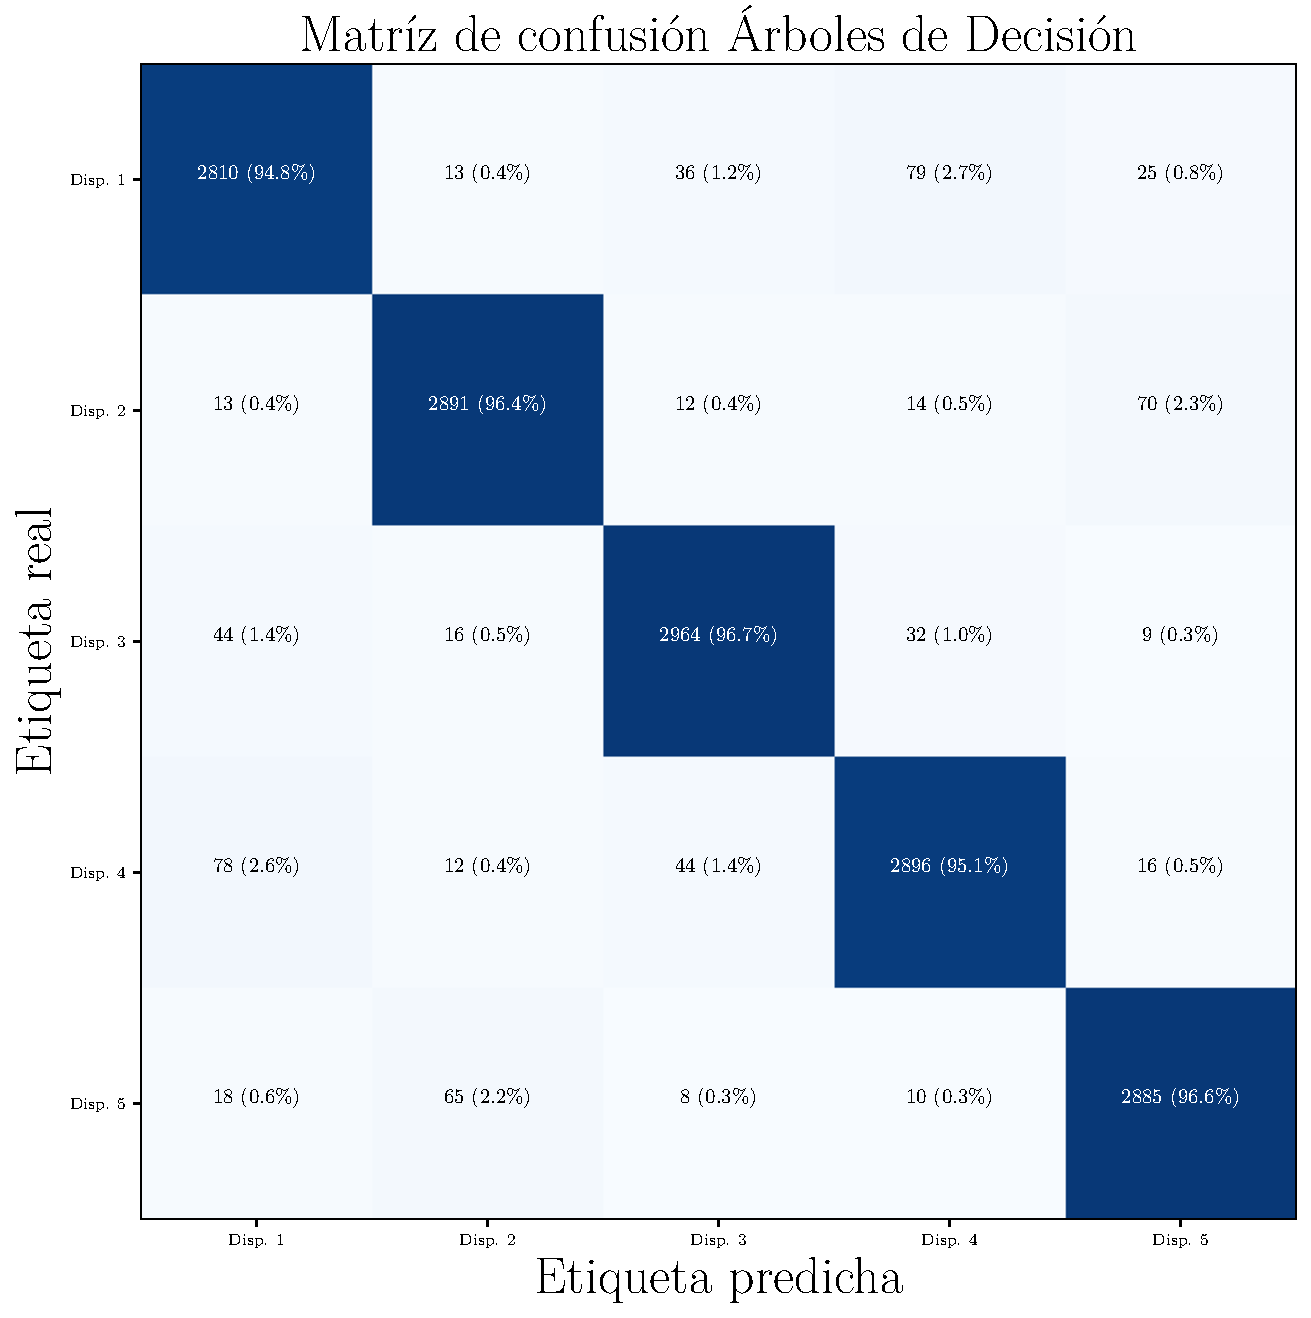
\includegraphics[width=0.4\textwidth]{../Python/plots/parallel/decision_tree_matrix}} & \subfloat{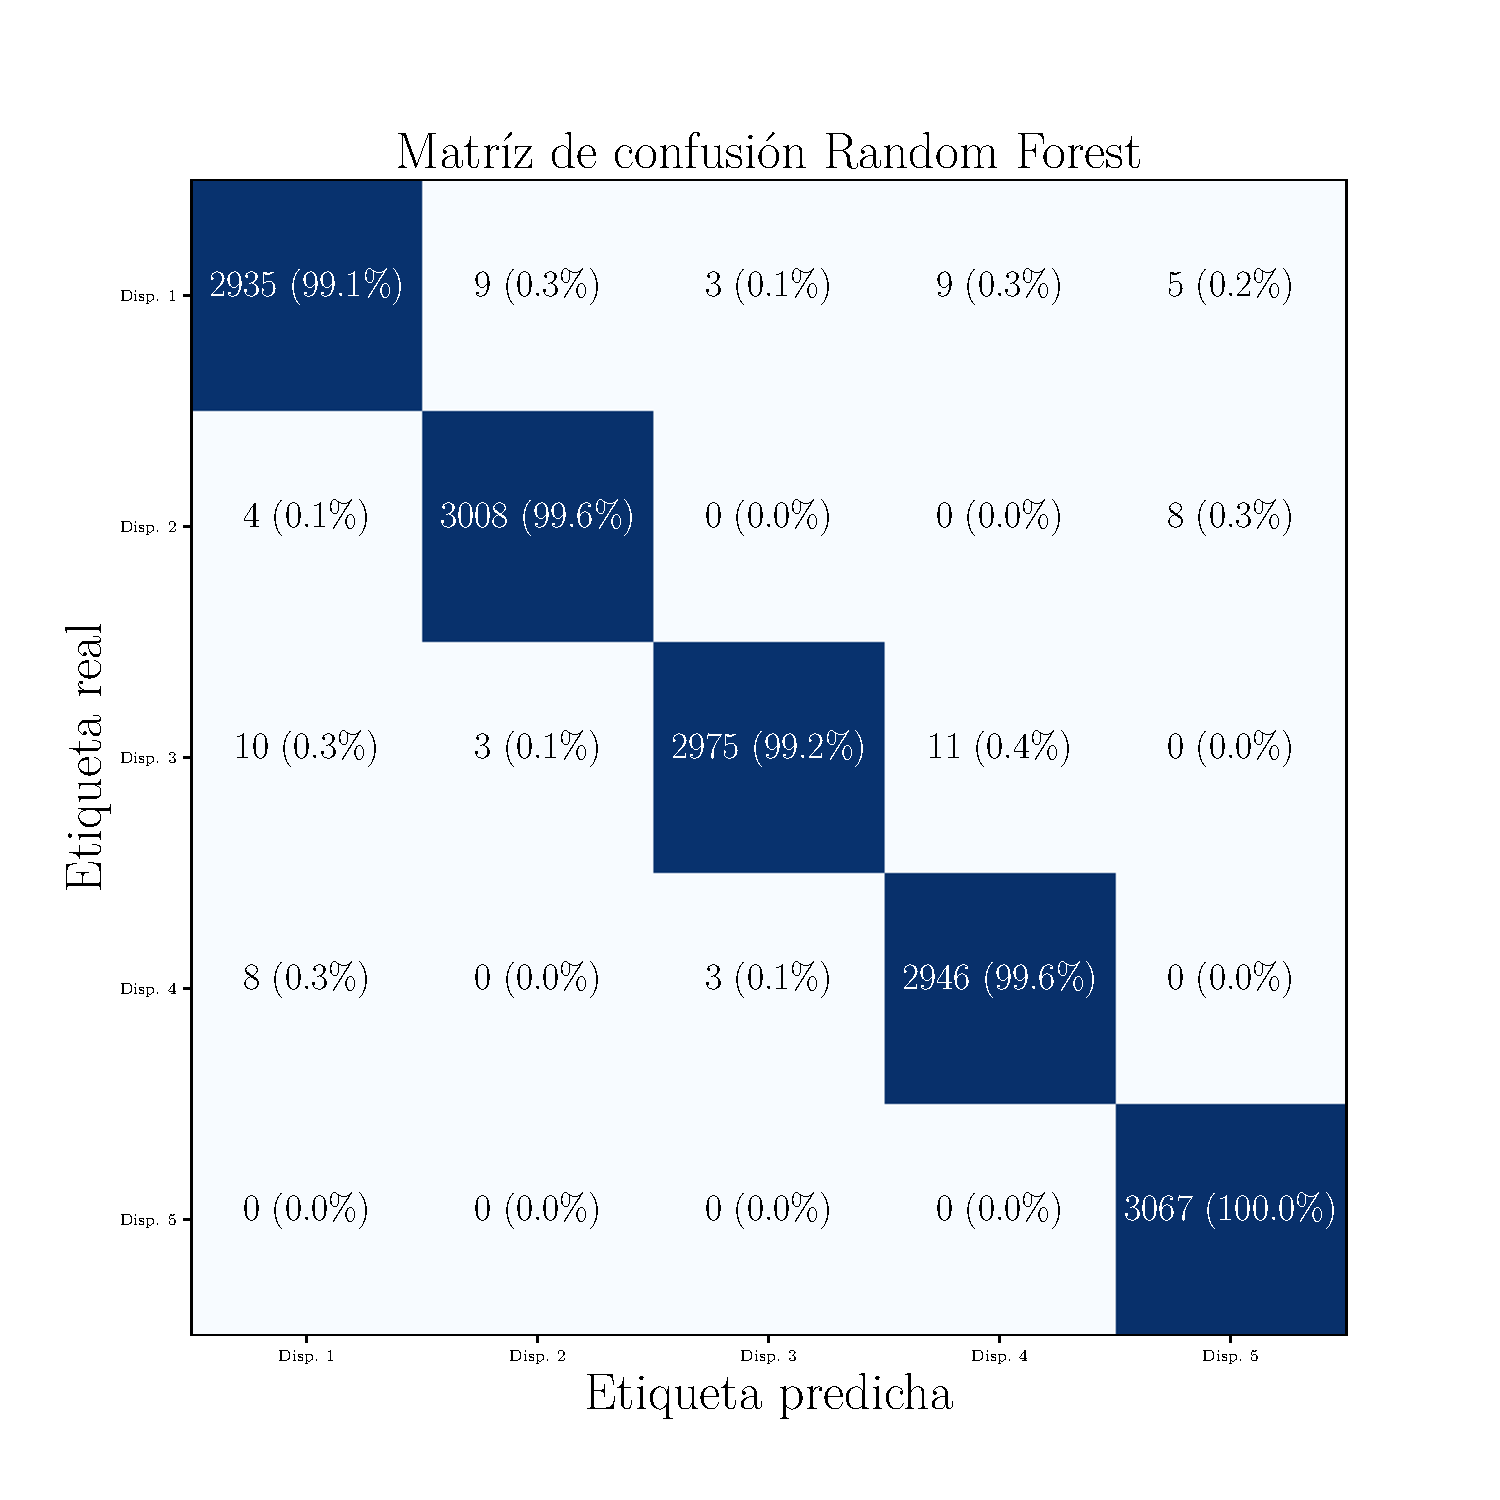
\includegraphics[width=0.4\textwidth]{../Python/plots/parallel/random_forest_matrix}} & \multirow{3}{*}[8em]{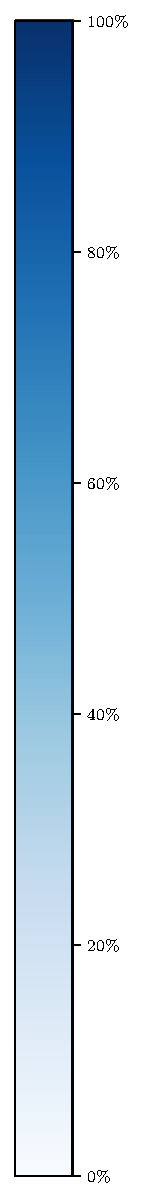
\includegraphics[scale=0.75]{../Python/plots/parallel/colorbar_matrices}} \\
        \subfloat{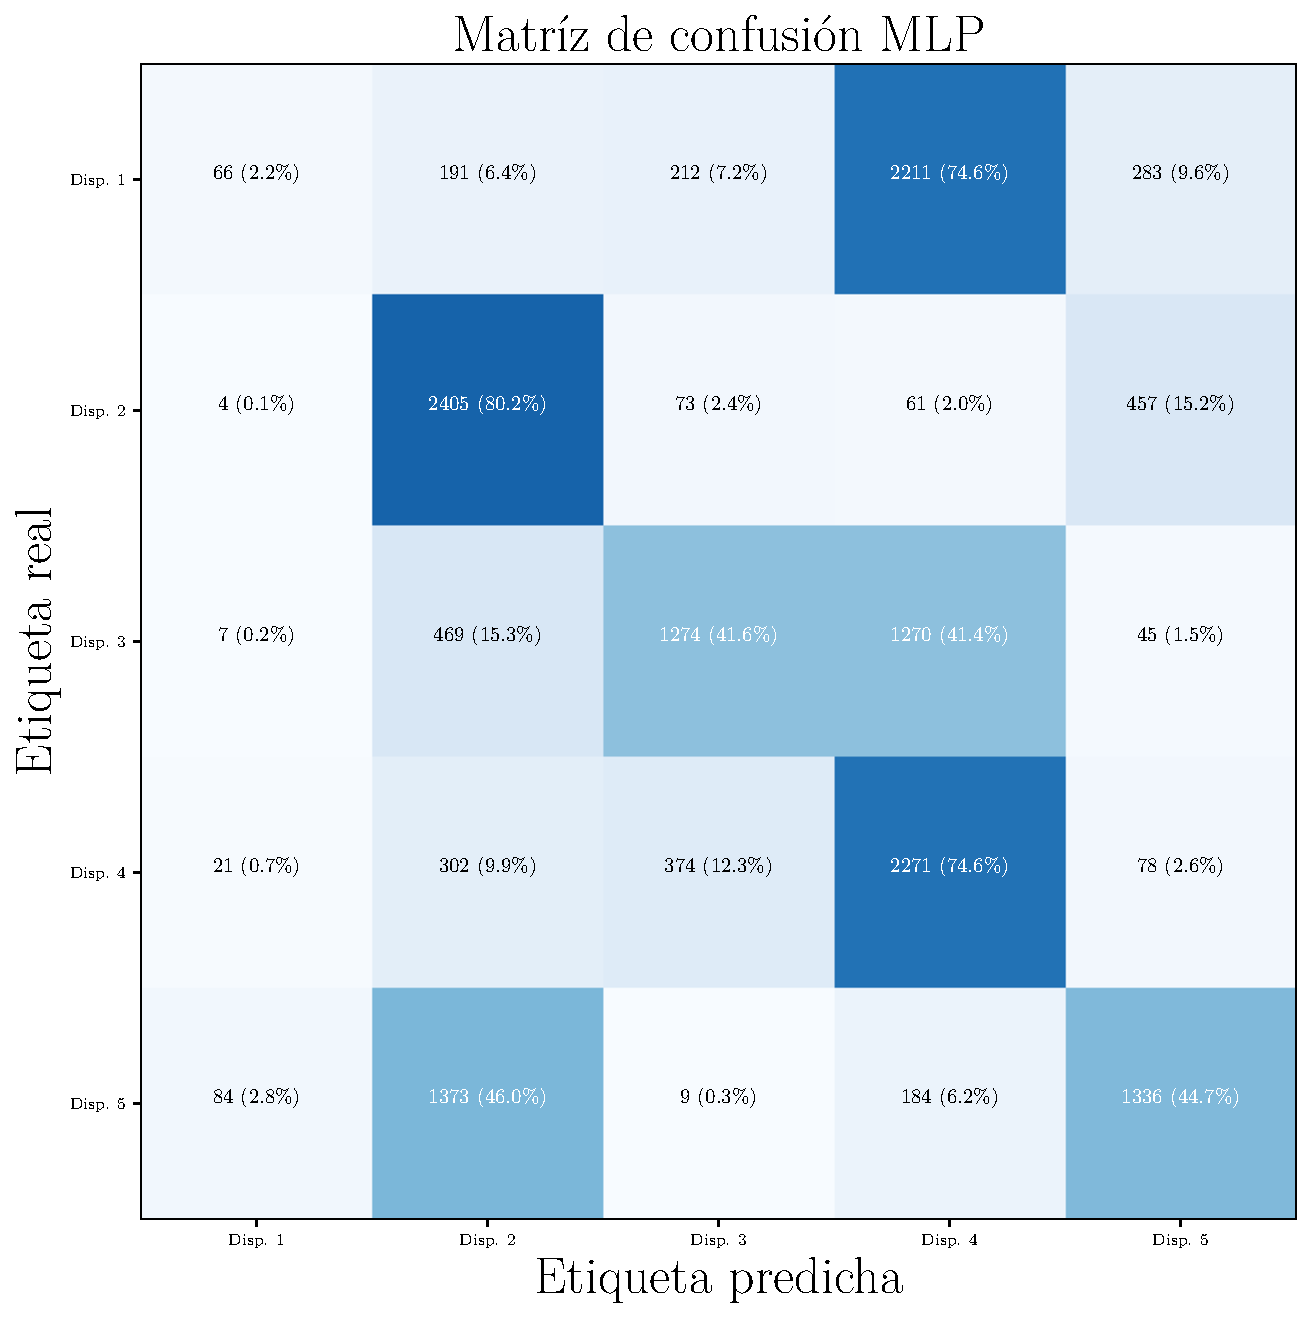
\includegraphics[width=0.4\textwidth]{../Python/plots/parallel/mlp_matrix}} & \subfloat{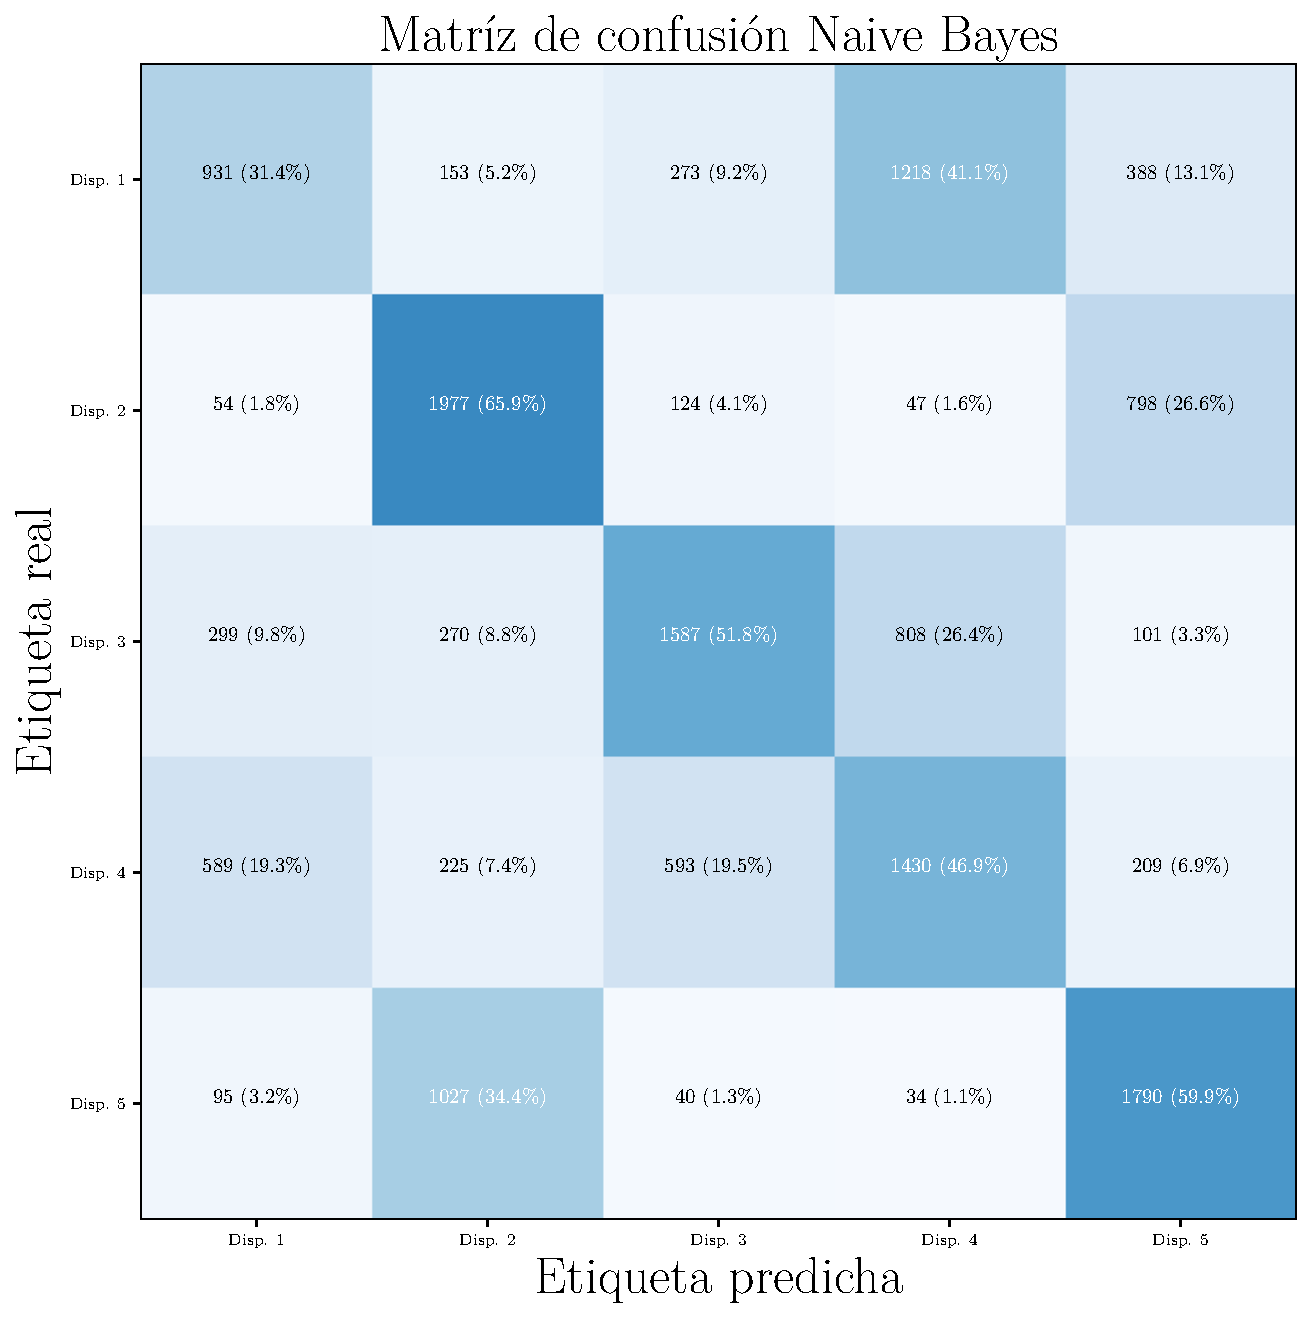
\includegraphics[width=0.4\textwidth]{../Python/plots/parallel/naive_bayes_matrix}} &  \\
        \subfloat{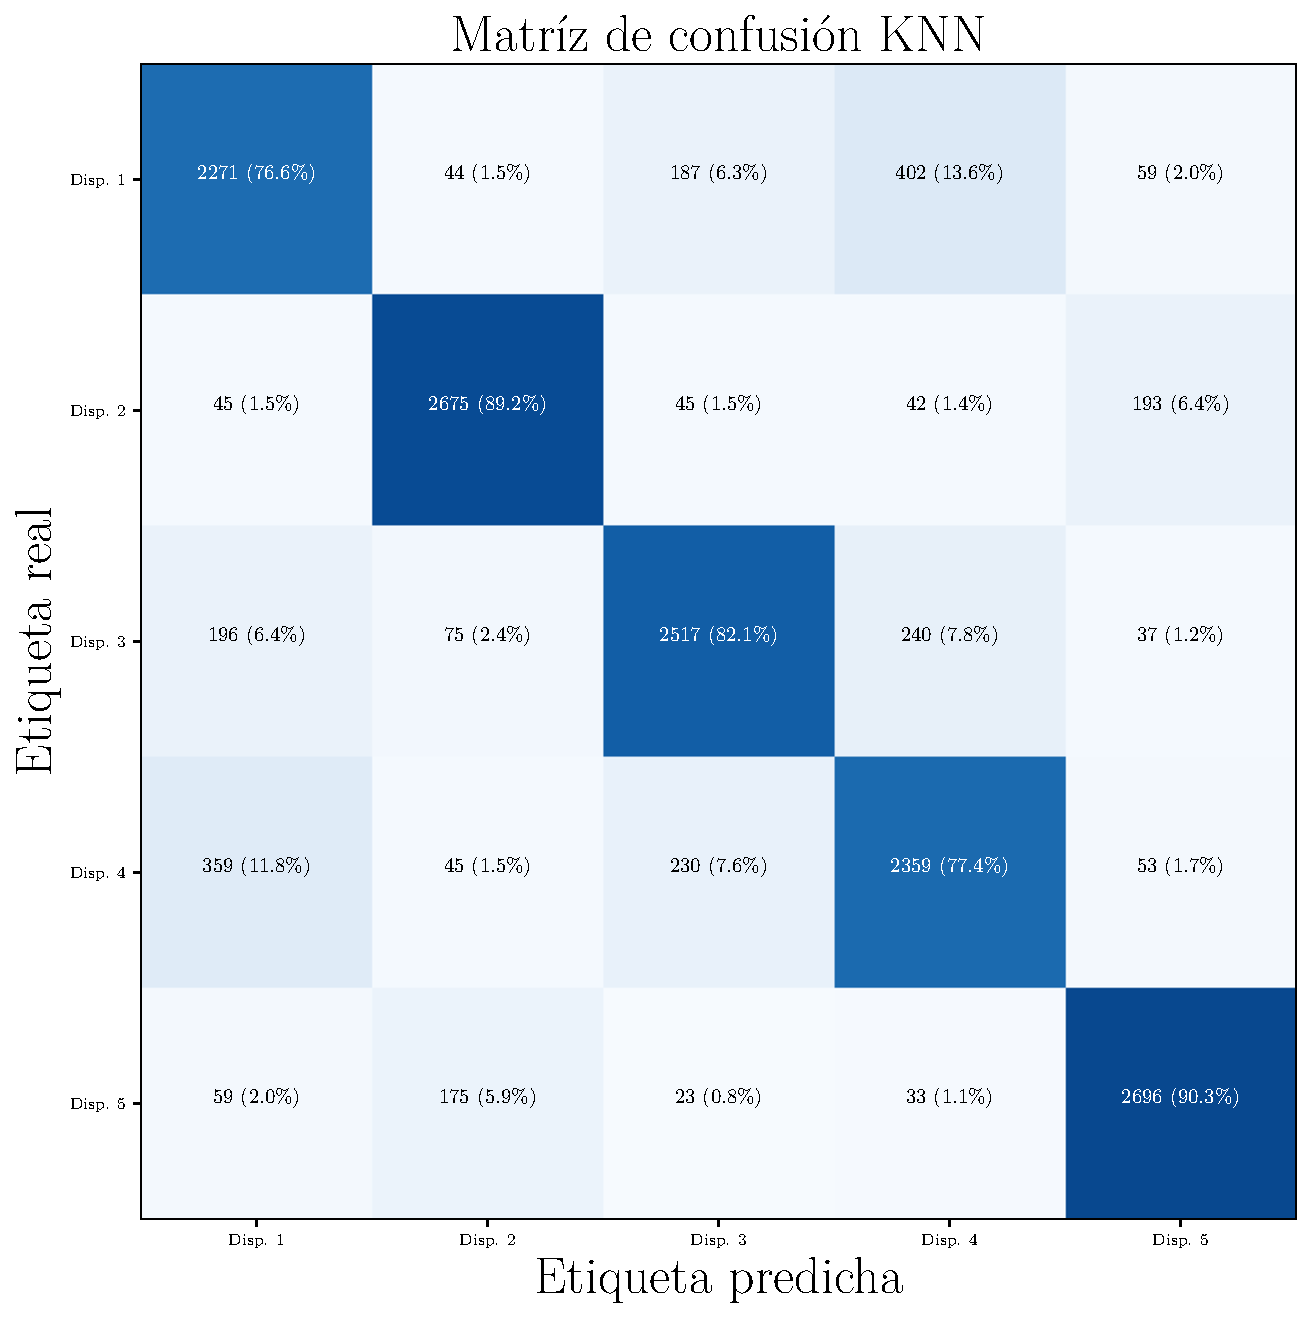
\includegraphics[width=0.4\textwidth]{../Python/plots/parallel/knn_matrix}} & \subfloat{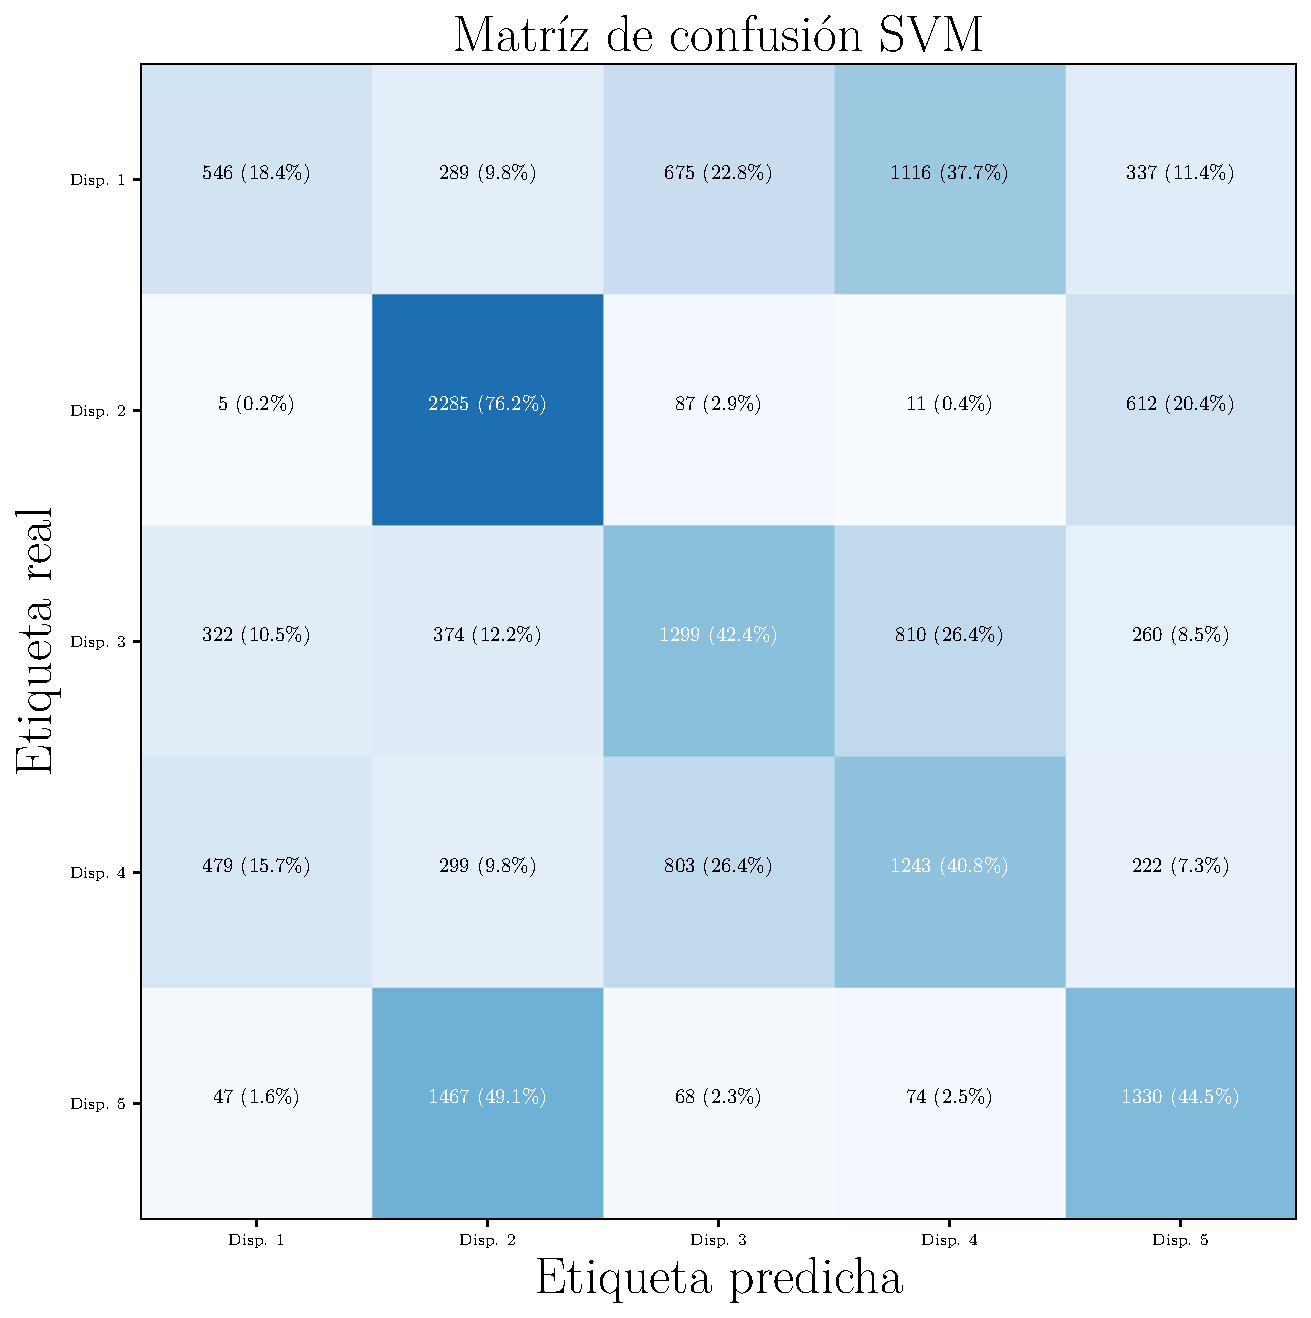
\includegraphics[width=0.4\textwidth]{../Python/plots/parallel/svm_linear_matrix}} & \\
    \end{tabular}
    \caption{Matrices de confusión con datos de la muestra paralela}
    \label{fig:confusion_matrices_parallel}
\end{figure}

Es fácil ver en la Fig. \ref{fig:confusion_matrices_parallel} que los modelos basados en árboles aciertan prácticamente en la totalidad de las ocasiones, en particular, el algoritmo de random forest es el que mejores resultados consigue ($\sim 99.5\%$). Por esta razón se entrenará un modelo de random forest con los hiperparámetros ajustados anteriormente con la totalidad de los datos de entrenamiento. Los resultados obtenidos se pueden ver en la matriz de confusión resultante (Fig. \ref{fig:final_matrix}). Con estos resultados se tiene un valor final de accuracy de 99.44\%.

\begin{figure}[H]
    \centering
    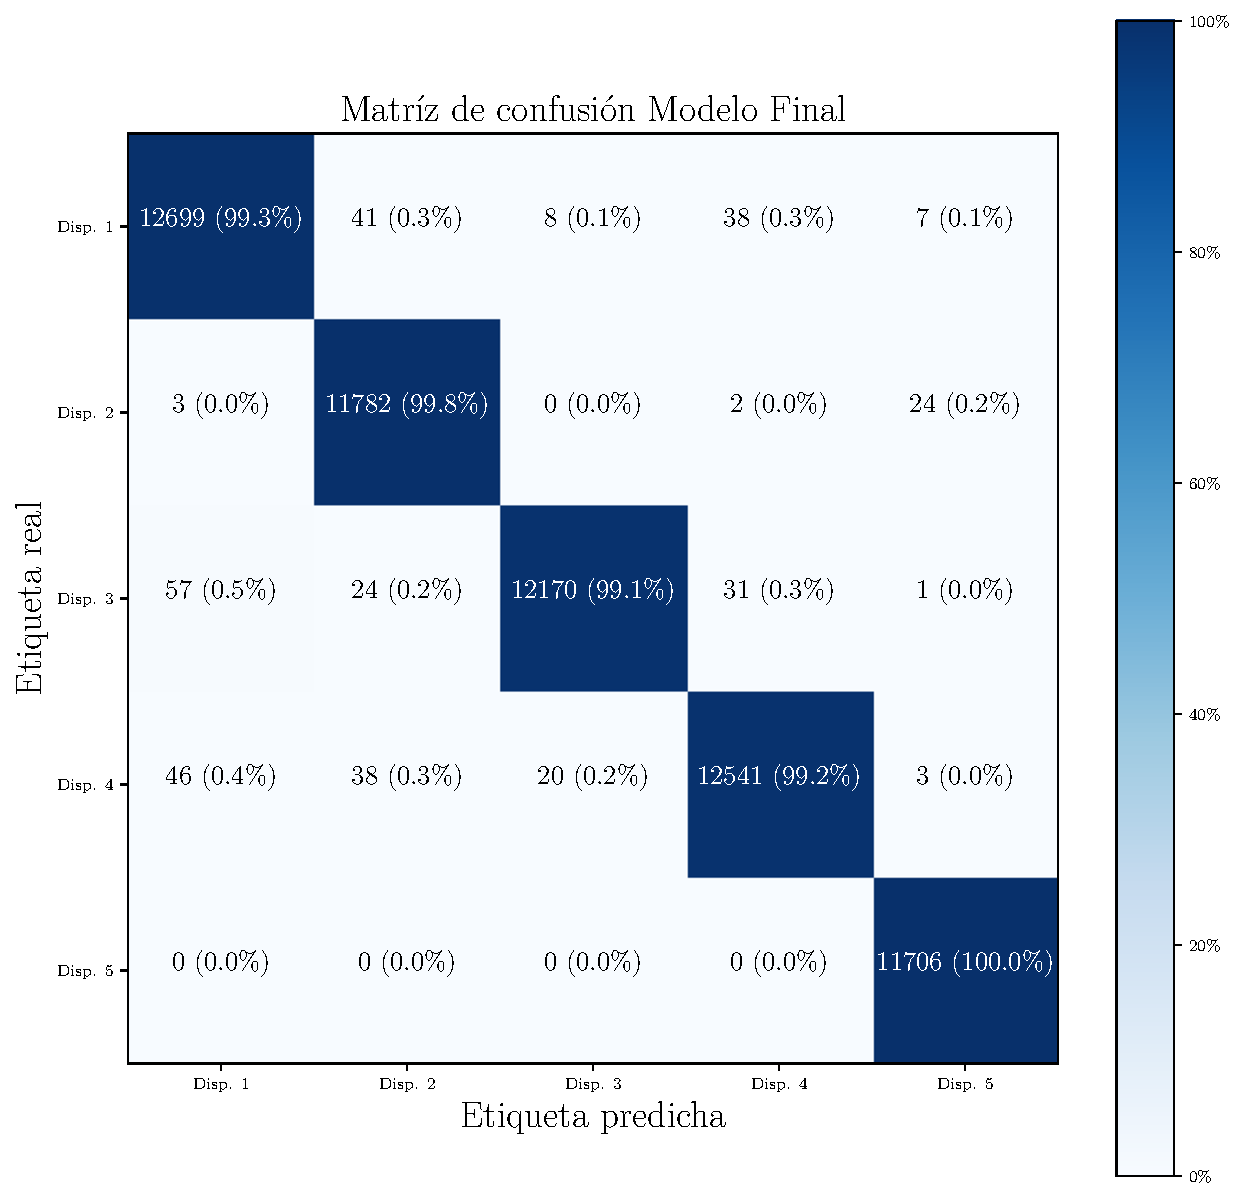
\includegraphics[scale=0.3]{../Python/plots/parallel/final_model_matrix}
    \caption{Matríz de confusión del modelo final}
    \label{fig:final_matrix}
\end{figure}
